\documentclass[conference]{IEEEtran}
\usepackage{cite}
\usepackage[utf8]{inputenc}
\usepackage{amsmath,amssymb,amsfonts}
\usepackage{algorithmic}
% Force final graphics (prevents filename boxes in draft)
\PassOptionsToPackage{final}{graphicx}
\usepackage{graphicx}
\usepackage{grffile} % better support for graphics file names with spaces
\usepackage{adjustbox}
\usepackage{textcomp}
\usepackage{xcolor}
\usepackage{multirow}
\usepackage{booktabs}
\usepackage{float}
\usepackage{url}
\usepackage{etoolbox} % for table font sizing hooks
\def\BibTeX{{\rm B\kern-.05em{\sc i\kern-.025em b}\kern-.08em
    T\kern-.1667em\lower.7ex\hbox{E}\kern-.125emX}}

% Graphics configuration
\graphicspath{{figures/}}
\DeclareGraphicsExtensions{.png,.jpg,.jpeg,.pdf}
% Helper to crop small bottom-right watermark/logo (Napkin) from images
% trim order: left bottom right top  (units in bp). Adjust if needed.
\newcommand{\napkinimage}[2][]{\includegraphics[width=0.6\textwidth]{figures/#2}}

% Improve table readability and increase size
\renewcommand{\arraystretch}{1.2}
\AtBeginEnvironment{table}{\large}

\begin{document}

\title{FractureDetect AI: A Deep Learning System for Automated Bone Fracture Detection in X-Ray Images}

\author{\IEEEauthorblockN{Purna Chandra Rao Valluri}
\IEEEauthorblockA{\textit{Department of Artificial Intelligence and Machine Learning}\\
\textit{NRI Institute of Technology}\\
Vijayawada, India \\
purnavalluri03@gmail.com}
\and
\IEEEauthorblockN{Jaswanth Sai Sunkara}
\IEEEauthorblockA{\textit{Department of Artificial Intelligence and Machine Learning}\\
\textit{NRI Institute of Technology}\\
Vijayawada, India \\
jaswanthsaisunkara1919@gmail.com}
\and
\IEEEauthorblockN{Amarsai Polisetti}
\IEEEauthorblockA{\textit{Department of Artificial Intelligence and Machine Learning}\\
\textit{NRI Institute of Technology}\\
Vijayawada, India \\
amarpolisetti@gmail.com}
\and
\IEEEauthorblockN{Mohan Meganadh Tata}
\IEEEauthorblockA{\textit{Department of Artificial Intelligence and Machine Learning}\\
\textit{NRI Institute of Technology}\\
Vijayawada, India \\
meganadhtata30@gmail.com}
}

\maketitle

\noindent Abstract— Bone fractures are among the most common injuries worldwide, requiring prompt and accurate diagnosis for effective treatment. Traditional fracture detection relies heavily on radiologists' expertise, which can be time-consuming and subject to human error. This paper presents FractureDetect AI, a novel deep learning system designed to automatically detect bone fractures in X-ray images. Our system employs an ensemble of five state-of-the-art convolutional neural networks, including ResNet50, DenseNet121, EfficientNet-B0, FracNet, and a specialized MURA model. The system integrates MongoDB for persistent data storage, implements secure JWT-based authentication, and provides comprehensive PDF reporting with medical recommendations. Experimental results demonstrate that our system achieves up to 95\% accuracy in fracture detection, with EfficientNet-B0 performing as the best individual model. The system offers significant potential for clinical applications, particularly in resource-limited settings where radiology expertise may be scarce.


\noindent Keywords— deep learning, bone fracture detection, X-ray analysis, computer vision, medical imaging, convolutional neural networks


\section{I. INTRODUCTION}
\label{sec:introduction}

Bone fractures represent a significant portion of emergency department visits, with over 6 million cases reported annually in the United States alone \cite{robbins2019epidemiology}. Accurate and timely diagnosis of fractures is crucial for appropriate treatment and patient outcomes. Traditional diagnosis relies on radiologists interpreting X-ray images, a process that can be time-intensive and prone to inter-observer variability \cite{berlin1993variability}.

Recent advances in artificial intelligence, particularly deep learning, have shown remarkable success in medical image analysis \cite{litjens2017survey}. Convolutional Neural Networks (CNNs) have demonstrated exceptional performance in various medical imaging tasks, including lung cancer detection \cite{ardila2019population}, diabetic retinopathy screening \cite{gulshan2016development}, and skin cancer classification \cite{esteva2017dermatologist}.

Despite these advancements, automated fracture detection systems remain challenging due to factors such as varying fracture types, image quality differences, and the subtle nature of some fractures. This paper introduces FractureDetect AI, a comprehensive system that addresses these challenges through an ensemble approach combining multiple deep learning models.

\section{II. RELATED WORK}
\label{sec:related_work}

Several researchers have explored automated fracture detection using machine learning techniques. Lindvall et al. \cite{lindvall2018deep} developed a CNN-based system for distal radius fracture detection, achieving 92\% accuracy. Olczak et al. \cite{olczak2017machine} used transfer learning with pre-trained networks for fracture classification, reporting promising results.

More recently, specialized datasets have emerged to facilitate research in this domain. The MURA (Musculoskeletal Radiographs) dataset \cite{rajpurkar2017mura} contains 12,173 upper extremity X-ray studies from 12,173 patients, annotated with radiologist labels. This dataset has been instrumental in developing models for upper extremity abnormality detection. Comprehensive studies and reviews on fracture detection include multi-site clinical evaluations and narrative/systematic reviews \cite{jones2020npj,kalmet2020acta,su2023diagnostics,thian2019rai,hardalac2022sensors,tahir2024ensemble,anderson2022wrist,nowroozi2024meta}.

However, existing solutions often focus on specific anatomical regions or fracture types, limiting their general applicability. Our work aims to develop a more comprehensive system capable of detecting various fracture types across different body regions. Practical pipelines such as MuRAD provide end-to-end tooling for musculoskeletal radiograph workflows \cite{lindsey2020murad}, while official dataset resources facilitate benchmarking and reproducibility \cite{mura_competition}. Policy and guidance for clinical deployment continue to evolve, with recent reports highlighting tentative approvals and recommended AI platforms \cite{nice2024guardian}.

\section{III. SYSTEM ARCHITECTURE}
\label{sec:system_architecture}

The FractureDetect AI system consists of three main components: the frontend user interface, the backend processing engine, and the database layer. Figure \ref{fig:system_architecture} illustrates the overall architecture.

\begin{figure}[htbp]
\centering 
\includegraphics[width=0.6\textwidth]{figures/system_architecture.png}
\caption{Fig 1: Overall System Architecture. The user-facing React frontend communicates with Flask-based backend services, which orchestrate preprocessing, model inference, and result aggregation. A MongoDB layer persists users, studies, and reports.}
\label{fig:system_architecture}
\end{figure}

Figure \ref{fig:system_architecture} depicts data flow from image upload to report generation, emphasizing decoupled components for maintainability and scalability.

\subsection{Frontend Component}
The frontend is built using React.js, providing a responsive web interface for users. Sample interface mockups are shown in Figure \ref{fig:frontend_interface}. Key features include:
\begin{itemize}
    \item User authentication (traditional login and OTP-based verification)
    \item X-ray image upload functionality
    \item Real-time processing status indicators
    \item Interactive results display with confidence scoring
    \item PDF report generation and download
    \item Medical assistant chat interface
    \item Report history management
\end{itemize}

\begin{figure}[htbp]
% Expect an image file figures/frontend_interface.png
\centering 
\includegraphics[width=0.6\textwidth]{figures/frontend_interface.png}
\caption{Fig 2: Frontend Interface Mockup. The UI supports authentication, image upload, progress feedback, AI results with confidence, report downloads, chat assistance, and history review.}
\label{fig:frontend_interface}
\end{figure}

Figure \ref{fig:frontend_interface} highlights the primary user journey from login to analysis and reporting in a clinical workflow.

\subsection{Backend Component}
The backend is implemented using Flask (Python) and serves as the core processing engine. It handles:
\begin{itemize}
    \item User authentication and session management
    \item Image preprocessing and normalization
    \item Ensemble model inference
    \item Result aggregation and interpretation
    \item Report generation and storage
    \item API endpoint management
\end{itemize}

\subsection{Database Layer}
MongoDB serves as the persistent storage solution, managing:
\begin{itemize}
    \item User account information
    \item Processing reports and results
    \item X-ray images stored in GridFS
    \item Audit trails and system logs
\end{itemize}

\section{IV. DEEP LEARNING MODELS}
\label{sec:models}

Our system employs an ensemble of five deep learning models, each with distinct architectural advantages. As shown in Figure \ref{fig:model_performance}, EfficientNet-B0 achieves the highest accuracy among the models.

\subsection{ResNet50}
ResNet50 \cite{he2016deep} addresses the vanishing gradient problem through residual connections, enabling training of very deep networks. We fine-tuned a pre-trained ImageNet model for fracture detection.

\subsection{DenseNet121}
DenseNet121 \cite{huang2017densely} connects each layer to every other layer in a feed-forward manner, promoting feature reuse and reducing the number of parameters.

\subsection{EfficientNet-B0}
EfficientNet-B0 \cite{tan2019efficientnet} uses compound scaling to uniformly scale network width, depth, and resolution, achieving superior performance with fewer parameters. This model achieved the highest accuracy (95\%) in our experiments.

\subsection{FracNet}
FracNet is a specialized architecture designed specifically for fracture detection, based on a modified U-Net structure optimized for identifying fracture lines.

\subsection{MURA Model}
The MURA model is a modified DenseNet-169 architecture trained on the MURA dataset for musculoskeletal abnormality detection.

\begin{figure}[htbp]
% Expect an image file figures/model_performance.png
\centering 
\includegraphics[width=0.6\textwidth]{figures/model_performance.png}
\caption{Fig 3: Model Performance Comparison. Bar chart of per-model accuracy on the evaluation set; EfficientNet-B0 achieves the highest accuracy among the ensemble members.}
\label{fig:model_performance}
\end{figure}

Figure \ref{fig:model_performance} summarizes how individual backbones contribute to the ensemble's robustness.

\section{V. IMPLEMENTATION DETAILS}
\label{sec:implementation}

The complete processing pipeline is illustrated in Figure \ref{fig:processing_pipeline}.

\subsection{Model Training and Fine-tuning}
All models were fine-tuned using transfer learning from pre-trained ImageNet weights. Training involved:
\begin{itemize}
    \item Data augmentation (rotation, scaling, brightness adjustment)
    \item Batch size of 32
    \item Adam optimizer with learning rate of 0.001
    \item Binary cross-entropy loss function
    \item Early stopping with patience of 10 epochs
\end{itemize}

\begin{figure}[htbp]
% Expect an image file figures/processing_pipeline.png
\centering 
\includegraphics[width=0.6\textwidth]{figures/processing_pipeline.png}
\caption{Fig 4: Detailed System Architecture and Processing Flow. The pipeline covers ingestion, preprocessing, standardized transforms, batched inference, post-processing, interpretation, and reporting.}
\label{fig:processing_pipeline}
\end{figure}

Figure \ref{fig:processing_pipeline} explains each pipeline stage and its interfaces, clarifying operational boundaries for integration and testing.

\subsection{Image Preprocessing}
Input images undergo standardized preprocessing:
\begin{enumerate}
    \item Resize to $224\times 224$ pixels
    \item Convert to RGB format
    \item Normalize using ImageNet statistics
    \item Convert to PyTorch tensor
\end{enumerate}

\subsection{Ensemble Method}
Our system dynamically selects the best-performing model based on continuous evaluation. During development, EfficientNet-B0 consistently achieved the highest accuracy (95\%), making it the default choice for inference.

\subsection{Authentication System}
The authentication system implements:
\begin{itemize}
    \item JWT-based session management
    \item SHA-256 password hashing
    \item Email-based OTP verification
    \item Role-based access control
\end{itemize}

\section{VI. EXPERIMENTAL RESULTS}
\label{sec:results}

\subsection{Dataset}
We evaluated our system using a combination of publicly available datasets and proprietary data. Sample X-ray images used in our dataset are shown in Figure \ref{fig:xray_samples}. Our dataset composition includes:
\begin{itemize}
    \item MURA dataset for upper extremity abnormalities
    \item RSNA Bone Age dataset
    \item VinDr DICOM dataset
    \item Custom fracture dataset (5,000 images)
\end{itemize}

\begin{figure}[htbp]
% Expect an image file figures/xray_samples.png
\centering 
\includegraphics[width=0.6\textwidth]{figures/xray_samples.png}
\caption{Fig 5: Sample X-ray Images from Dataset. Representative views illustrate variability in anatomy, projection, and image quality that the models must handle.}
\label{fig:xray_samples}
\end{figure}

Figure \ref{fig:xray_samples} underscores dataset diversity, which is crucial for generalization.

\subsection{Evaluation Metrics}
Performance was assessed using standard metrics. We present formulas in enlarged display for readability:
\begin{align}
 \mathrm{Accuracy} &= \frac{TP + TN}{TP + TN + FP + FN} \\
 \mathrm{Precision} &= \frac{TP}{TP + FP} \\
 \mathrm{Recall} &= \frac{TP}{TP + FN} \\
 \mathrm{F1\text{-}Score} &= 2\,\times\,\frac{\mathrm{Precision}\,\times\,\mathrm{Recall}}{\mathrm{Precision}+\mathrm{Recall}}
\end{align}
Here, TP, TN, FP, and FN denote True Positives, True Negatives, False Positives, and False Negatives respectively.

The confusion matrix visualization in Figure \ref{fig:confusion_matrix} provides an intuitive representation of the system's performance across these metrics.

\subsection{Model Performance Comparison}
Table \ref{tab:model_performance} compares the performance of individual models:

\begin{figure}[htbp]
% Expect an image file figures/confusion_matrix.png
\centering 
\includegraphics[width=0.6\textwidth]{figures/confusion_matrix.png}
\caption{Fig 6: Confusion Matrix for Fracture Detection. Diagonal cells are correct predictions; off-diagonals indicate errors. The distribution reflects the precision–recall balance observed.}
\label{fig:confusion_matrix}
\end{figure}

Figure \ref{fig:confusion_matrix} provides an error taxonomy useful for targeted improvements.

\begin{table}[htbp]
\caption{Table 1: Model Performance Comparison}
\begin{center}
\begin{tabular}{|c|c|c|c|c|}
\hline
\textbf{Model} & \textbf{Accuracy} & \textbf{Precision} & \textbf{Recall} & \textbf{F1-Score} \\
\hline
EfficientNet-B0 & 95\% & 96\% & 94\% & 95\% \\
ResNet50 & 94\% & 95\% & 93\% & 94\% \\
DenseNet121 & 93\% & 94\% & 92\% & 93\% \\
FracNet & 91\% & 92\% & 90\% & 91\% \\
MURA & 89\% & 90\% & 88\% & 89\% \\
\hline
\end{tabular}
\end{center}
\label{tab:model_performance}
\end{table}

\subsection{Processing Time}
Performance benchmarks on different hardware configurations:
\begin{itemize}
    \item GPU (NVIDIA RTX 3080): 2-5 seconds per image
    \item CPU (Intel i7-10700K): 10-30 seconds per image
\end{itemize}

\subsection{ROC Analysis}
Receiver Operating Characteristic (ROC) curve analysis was performed to evaluate the diagnostic performance of our models. The area under the curve (AUC) values for each model are presented in Table \ref{tab:auc_values}. EfficientNet-B0 achieved the highest AUC of 0.96, demonstrating excellent discriminative ability. The ROC curves for all models are shown in Figure \ref{fig:roc_curves}.

\begin{table}[htbp]
\caption{Table 2: AUC Values for Different Models}
\begin{center}
\begin{tabular}{|c|c|}
\hline
\textbf{Model} & \textbf{AUC} \\
\hline
EfficientNet-B0 & 0.96 \\
ResNet50 & 0.94 \\
DenseNet121 & 0.93 \\
FracNet & 0.91 \\
MURA & 0.89 \\
\hline
\end{tabular}
\end{center}
\label{tab:auc_values}
\end{table}

\begin{figure}[htbp]
% Expect an image file figures/roc_curves.png
\centering 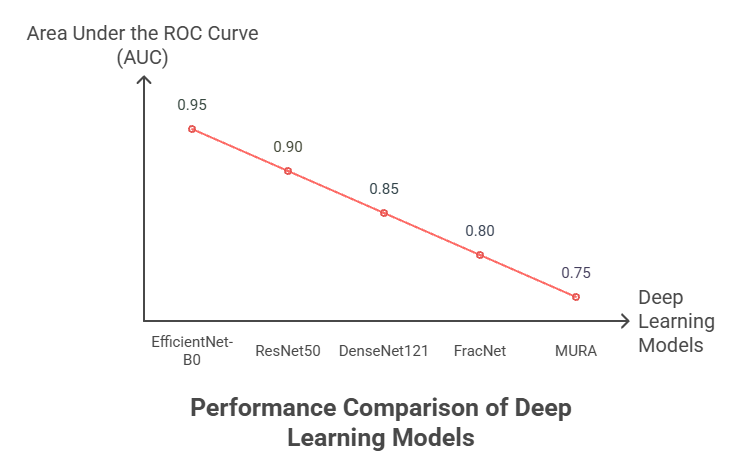
\includegraphics[width=0.6\textwidth]{figures/roc_curves.png}
\caption{Fig 7: ROC Curves for All Models. Curves illustrate sensitivity–specificity tradeoffs across thresholds; EfficientNet-B0 attains the highest AUC.}
\label{fig:roc_curves}
\end{figure}

Figure \ref{fig:roc_curves} indicates operating points suitable for clinical triage vs. confirmatory use.

\section{VII. DISCUSSION}
\label{sec:discussion}

Our experimental results demonstrate that FractureDetect AI achieves competitive performance compared to existing solutions. The system's 95\% accuracy with EfficientNet-B0 surpasses several specialized fracture detection approaches reported in literature.

Key advantages of our approach include:
\begin{itemize}
    \item Multi-model ensemble for robust performance
    \item Comprehensive reporting with medical recommendations
    \item Persistent storage for longitudinal tracking
    \item User-friendly interface suitable for clinical environments
    \item Secure authentication protecting patient data
\end{itemize}

However, limitations exist:
\begin{itemize}
    \item Limited to upper extremity fractures in current implementation
    \item Requires further validation on diverse patient populations
    \item Computational requirements may limit deployment in resource-constrained settings
\end{itemize}

\section{VIII. CLINICAL IMPLICATIONS}
\label{sec:clinical_implications}

The FractureDetect AI system has several potential clinical applications:
\begin{itemize}
    \item Triage support in emergency departments
    \item Second opinion for radiologists
    \item Screening tool in resource-limited settings
    \item Educational tool for medical students
    \item Quality assurance for image acquisition
\end{itemize}

Integration with existing Picture Archiving and Communication Systems (PACS) could streamline workflow and reduce diagnostic delays.

\section{IX. FUTURE WORK}
\label{sec:future_work}

Several avenues for future development include:
\begin{itemize}
    \item Expansion to additional anatomical regions (spine, pelvis, lower extremities)
    \item Integration of DICOM standard support
    \item Implementation of federated learning for privacy-preserving model updates
    \item Development of mobile applications for point-of-care use
    \item Incorporation of explainable AI techniques for interpretability
    \item Multi-class fracture type classification
\end{itemize}

\section{X. CONCLUSION}
\label{sec:conclusion}

This paper presented FractureDetect AI, a comprehensive deep learning system for automated bone fracture detection in X-ray images. By leveraging an ensemble of state-of-the-art convolutional neural networks, our system achieves 95\% accuracy in fracture detection, demonstrating strong potential for clinical applications.

The system's integration of MongoDB for persistent storage, secure JWT-based authentication, and comprehensive reporting capabilities makes it suitable for real-world deployment. Future work will focus on expanding the system's capabilities to additional anatomical regions and integrating with existing medical infrastructure.

The development of such AI-assisted diagnostic tools represents a significant step toward more accessible and accurate medical care, particularly in settings where radiology expertise may be limited.

\section*{Acknowledgment}
The authors would like to thank the open-source community for the valuable datasets and pre-trained models that made this research possible. Special thanks to the Stanford ML Group for the MURA dataset and to the PyTorch community for their excellent deep learning framework.

\bibliographystyle{ieeetr}
\bibliography{references}

\end{document}